\documentclass[12pt,a4paper,titlepage,spanish]{article} 
\usepackage{babel}
\usepackage [T1]{fontenc}
\usepackage [latin1]{inputenc}
\usepackage{graphicx}
\usepackage{amssymb}
\usepackage{amsmath}
\usepackage{setspace}
\usepackage{epsfig}
\usepackage{enumerate}
\usepackage{float}
\usepackage{array}
\usepackage{cancel}
%\usepackage{arcs}
\usepackage[usenames,dvipsnames]{color}
	  \oddsidemargin 0in
      \textwidth 6.75in
      \topmargin 0in
      \textheight 10.0in
      \parindent 0em
      \parskip 2ex
\usepackage{anysize}
\marginsize{3cm}{2cm}{1.0cm}{1.0cm}
\pagestyle{plain}
\title{
\begin{Large}
 \begin{center}
		\underline{Informe Simulaciones TP10: M�todo de transformada inversa} \\
		\underline{Generaci�n de n�meros aleatorios con distribuciones no uniformes}\\
		\underline{Curso: } 6to 1ra\\
		\underline{Turno: } Noche\\
		\underline{CPU: } Intel Core 2 Duo E6600\\
      \end{center}
\end{Large}
}
\author{Vileri�o, Silvio}

\begin{document}
\maketitle
\setcounter{page}{2}
\tableofcontents
\newpage

\subsection{Introducci�n}
En esta simulaci�n se desarrolla el m�todo de la transformada inversa para la generaci�n de n�meros aleatorios de distribuci�n de probabilidad no uniforme utilizando la funci�n o transformada inversa de la funci�n de distribuci�n.

\begin{equation*}
	\\Sea\left\lbrace
	  \begin{array}{l}
		\text{$ f(x) $ una funci�n definida en el intervalo } [ \alpha, \beta ] \\
		\text{$ x $ } \in \mathbb{R_a}  [ \alpha, \beta ]\\
	  \end{array}
	  \right.
\end{equation*}
Se desean generar $ K $ n�meros aleatorios donde $ \alpha=1 $ , $ \beta=10 $ dando un intervalo $ [1, 10] $ con una funci�n de distribuci�n o reparto del tipo $ f(x)=\frac{1}{x} $, de forma que la distribuci�n quede dada por $ f(x) $ y el
histograma adquiera la siguiente forma:\\
\begin{center}
	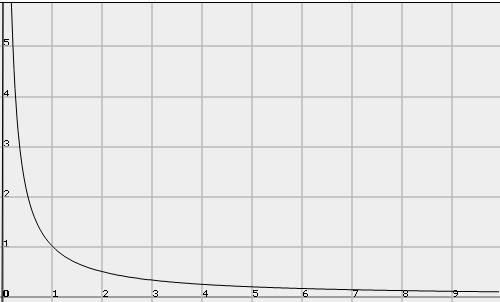
\includegraphics[scale=0.75]{images/Distribucion-1x.JPG}
\end{center}

Se procede a calcular $ N $, que indica la cantidad de puntos en un intervalo(estad�sticamente).
\begin{center}
 $ N=\int_\alpha^{\beta}\frac{1}{x} \: dx $
\end{center} 
Una vez calculado $ N $, se procede a calcular la funci�n $ g(x) $, que no es m�s que la funci�n $ f(x) $ normalizada por $ N $, lo cual nos da la probabilidad de aparici�n de $ x $ en el intervalo $ [ \alpha, \beta ] $ calculando $\int_\alpha^{\beta}g(x) \: dx  $\\
Teniendo esto en cuenta, podemos obtener las siguientes deducciones:\\
\begin{center}
	$ \int_\alpha^{\beta}g(x) \: dx= \int_\alpha^{\beta}\frac{f(x)}{N} \: dx=p(x) $ Donde p es la probabilidad de aparici�n de x. $ x \in  [ \alpha, \beta ]  $
\end{center} 
Si acotamos el intervalo a $ [\alpha, \gamma] $, obtenemos $ \int_\alpha^{\gamma}g(x) \: dx= \int_\alpha^{\gamma}\frac{f(x)}{N} \: dx=p(x) $ Podemos manejar los intervalos seg�n nos convenga pero esta ecuaci�n siempre nos dar� n�meros
en el intervalo $ [0,1] $ pudiendo establecer la siguiente igualdad:
\begin{center}
	$ \int_\alpha^{\gamma}g(x) \: dx=p(x)=Rnd $,  $ Rnd \in \mathbb{R_a} / 0 \leq Rnd \leq 1 $
\end{center} 
Entonces, si introducimos valores del intervalo $ [\alpha, \gamma] $ en $ p(x) $ obtenemos $ [0, 1] $.\\
Esto implica que:\\
\begin{center}
	 $ p : [\alpha, \gamma] \longrightarrow [0, 1] $\\
	 $ p ^{[-1]}: [0, 1] \longrightarrow [\alpha, X]  $
\end{center} 
Si ingresamos valores del intervalo $ [0, 1] $ en $ p^{[-1]} $ obtendremos un GNA con una distribuci�n dada por $ f(x) $
\begin{center}
	$ x=p^{[-1]}(Rnd)$
\end{center}
\underline{Ejemplo Practico:}\\
Funci�n $ f(x)=\frac{1}{x} $\\\\
Intervalo $ [\alpha, \beta ] = [0, 1] $\\\\
Se calcula $ N= \int_\alpha^{\beta}\frac{1}{x} \: dx = \int_1^{10}\frac{1}{x} \: dx = \ln(10) - \ln(1) = \ln(\frac{10}{1})$\\\\
$ N=\ln(10) $\\\\
$ g(x)=\frac{\frac{1}{x}}{\ln(10)} = \frac{1}{x.\ln(10)} $\\\\
$ \int_\alpha^{X}\frac{1}{x.\ln(10)} \: dx = \frac{1}{\ln(10)}.\ln(x) \left.\right|_{\alpha}^{X} $\\\\
$ \ln(x)  \left.\right|_{\alpha}^{\gamma}= \ln(\gamma)-\ln(\alpha) =\ln(\frac{X}{\alpha}) $\\\\\\
\begin{center}
$ y= \frac{\ln(\frac{\gamma}{\alpha})}{\ln(10)} $\\
$ y.\ln(10)=ln(\frac{\gamma}{\alpha}) $\\
%$ e^{\ln(10).y=\frac{\gamma}{\alpha}} $\\
$ \gamma= \alpha .e^{\ln(10).y} $ donde $ y=RND $\\
\end{center}
Funci�n inversa final:
\begin{center}
\textcolor{green}{$ X=\alpha.e^{\ln(\gamma).x}$ donde $ x=RND $}
\end{center}
Luego de realizar la simulaci�n, se obtuvieron los siguientes resultados: \\
\begin{itemize}
	\item Funcion $ f(x)=\frac{1}{x} $
	\item Intervalo $ [1, 10] $
	\item Cantidad de n�meros generados : 1000000
\end{itemize}
\begin{center}
	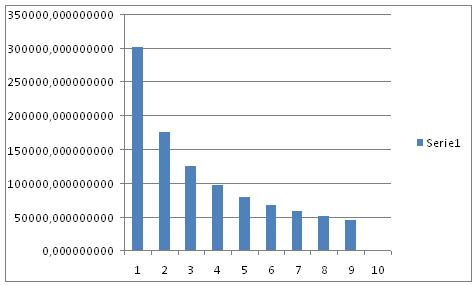
\includegraphics[scale=0.75]{images/Histograma.jpg}
\end{center}
\newpage
\subsection{Conclusi�n}
Se comprueba que por medio de este m�todo se pueden obtener distribuciones en funci�n de una tranformada cualquiera, en este caso $ f(x)=\frac{1}{x} $. Es un m�todo interesante y �til, ya que se puede utilizar para alimentar simulaciones estoc�sticas con alguna tendencia en particular, lo cual ampl�a las posibilidades de investigaci�n.
\end{document}